\chapter{Apps and their artefacts}~\label{chapter-apps-and-their-artefacts}
\julian{This chapter covers \uartefacts and \iartefacts. I'm currently drafting this chapter to try and work out what the major topics and groupings are, and then where the evidence I have fits. I'm currently inspired by \href{https://about.sourcegraph.com/blog/developer-productivity-thoughts}{A dev's thoughts on developer productivity}\citep{liu2022_a_devs_thoughts_onDeveloper_productivity} and the underlying spreadsheet of the findings is \href{https://docs.google.com/spreadsheets/d/1PcwJ6E_X6peCP1dBPADEAJXOBpnb4JY1gSGNyPSxedA/edit?usp=sharing}{here} and you should have access from your Google account if you are helping me with this thesis.}

The artefacts are a product, an outcome, of what developers do as they create and maintain their mobile apps. They include the source code of the codebase which evolves on an ongoing basis for active projects, any bug-tracking/bug-management system, outputs from builds including test results, outputs from mobile analytics. 

To some extent the artefacts reflect macro (big-picture) topics including ethics, scaling, data-pipelines, engineering tradeoffs, and decisions on using third-party code.


\section{Macro topics}

\textbf{Ethics:} Several of the development teams had to make explicit decisions whether to use mobile analytics and if so which one they would use. The Kiwix project team chose explicitly to exclude mobile analytics from their apps to reduce the potential for end users to be tracked and potentially imprisoned through their use of the app and Wikipedia content in particular~\footnote{The Kiwix project was developed to provide offline access to all of Wikipedia, it was then extended to support and provide lots of other content and material, nonetheless Wikipedia content is the one most likely to put end users at risk in some jurisdictions.} The Kiwix team did decide to use the platform-provided analytics from Google Play Console on the grounds that if the end-user had a) installed the Kiwix app from Google Play and b) had enabled (or at least not disabled) Google's collection of usage and performance data from their phones then the users were not being compromised by the devs using the analytics generated from the data those phones and tablets had provided.

The Catrobat team started by adding Fabric Crashlytics into their Pocket Code Android app several years before becoming a case study for this research. After seeing the results of applying the techniques from this research they choose to add Crashlytics to their iOS Pocket Code app and were also planning to use Firebase Analytics to record more granular usage data to both the Android and iOS apps. However, as a side-effect of migrating from the Fabric Analysis to Firebase Analysis - using the same client side SDK release they discovered they started receiving demographic data in tandem to the reliability analytics. Google then set a deadline where developers would need to replace the Fabric client side SDK with a similar one from Firebase to continue receiving any of the reports. The Catrobat team decided to stop using Crashlytics entirely rather than having demographics meta data collected by these SDKs in their apps. The Catrobat team had no objections to continuing to use the platform-provided analytics.

\textbf{Scaling}


\section{Normal and acceptable ranges of failures}
For the GTAF case study, the crash rates, as measured by Android Vitals, vary massively by release of the app (Al Quran (Tafsir \& by Word).\pending{A great deal more analysis is possible given the number of active apps and the ongoing access to Google Play Console.} 

Android Vitals does not report any failures in the GTAF taskinator app, which is created using React Native according to the development team. This is pertinent as similar behaviours in Android Vitals were observed for another app-centric case study, LocalHalo. 


\section{Improvements in crash rates}
For both Catrobat and Kiwix the hackathon and the post-hackathon bug fixes were highly effective in terms of cumulatively reducing the crash rate over several subsequent releases. % TODO Check whether the releases were contiguous.
The Catrobat case study replicated the improvements seen in the Kiwix case study and also the efficacy of using a hackathon as an immediate intervention. TODO discuss limitations of hackathons and forward link to the section on the useful half-life of hackathons. 


For Pocket Code, the improvements in the stability of the app were particularly encouraging as the project had already implemented many of `good' development practices.


\section{Discussion}\label{apps-and-artefacts-discussion-section}
Much of a developer's focus, perhaps unsurprisingly, is working with code and modifying code to achieve various objectives. An industry-focused article by Beyang Liu discusses the author's thoughts on developer productivity and introduces a term `\textbf{developer hertz}' as a measure of developer productivity~\citep{liu2022_a_devs_thoughts_onDeveloper_productivity} and defines it as once around the developer's inner loop (illustrated in Figure \ref{fig:developer-inner-loop-outer-loop}). This article provides a helpful context for the work of app developers where automated tests, use of mobile analytics, bug reproducibility, bug tracking, choosing third-party libraries, and various other activities emerged from the thematic analysis of the various findings pertaining to this research.

\begin{figure}
    \centering
    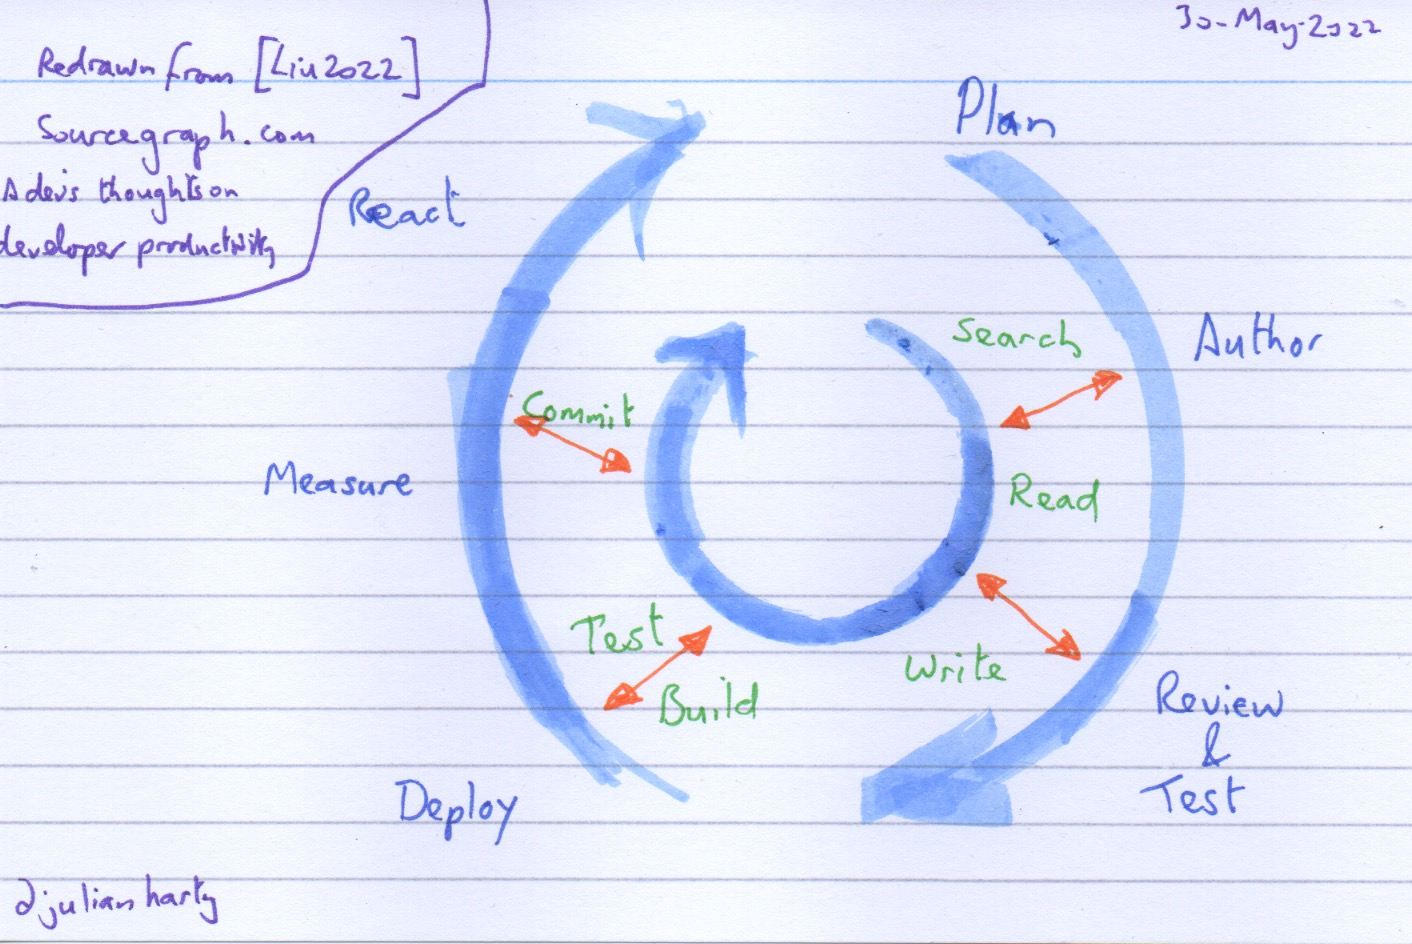
\includegraphics[width=12cm]{images/rough-sketches/developer-inner-loop-outer-loop.jpeg}
    \caption{Developer Inner Loop, Outer Loop\\ redrawn from \citep{liu2022_a_devs_thoughts_onDeveloper_productivity}}
    \label{fig:developer-inner-loop-outer-loop}
\end{figure}

\subsection{An iterative development lifecycle for app developers}
The research includes many findings that illustrate a conceptual iterative loop for app developers in terms of how their code is performing; to answer how's it doing in the real world. Figure \ref{fig:dev-app-reliability-iterative-loop} approximates various potential activities within this loop.

\begin{figure}
    \centering
    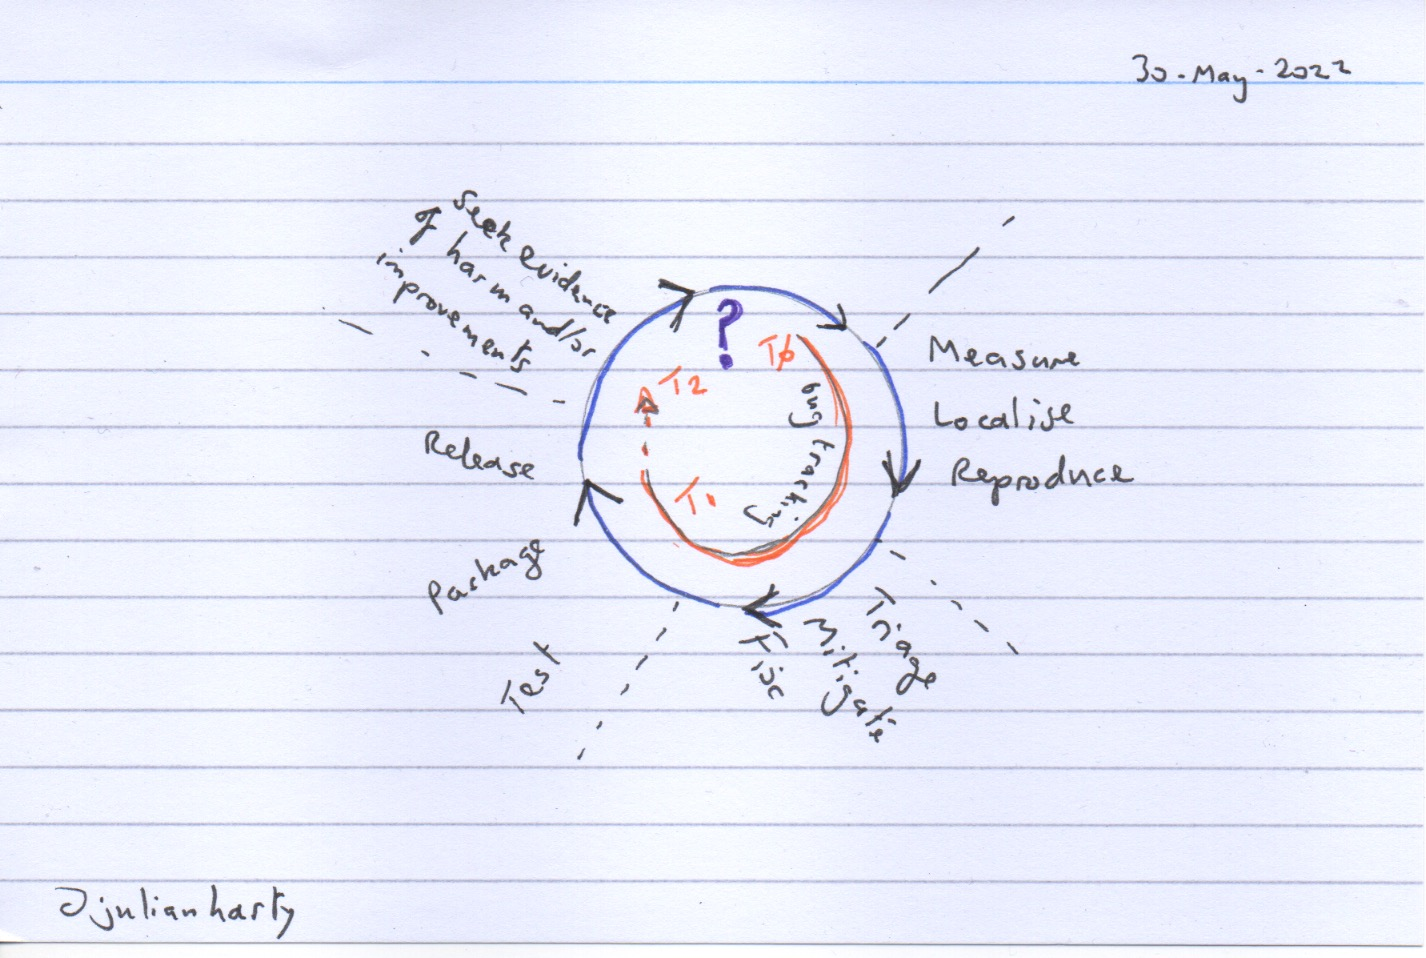
\includegraphics[width=12cm]{images/rough-sketches/dev-app-reliability-iterative-loop.jpeg}
    \caption{Developer's conceptual app reliability iterative loop}
    \label{fig:dev-app-reliability-iterative-loop}
\end{figure}

The loop starts with at the question-mark where the developers have a question about a flaw in the field related to their app's performance. They search for information which may include bug-localisation, adding logging to the app, and trying to reproduce the flaw using various techniques. They \emph{may} record the flaw in their issue tracking system, if so T0 marks the start of that bug in the bug tracking system.

They \emph{may} triage, mitigate, and/or attempt to fix the flaw, and if so they are likely to test the potential improvement(s), package the changes in a potential release and release it via the app store. Once the new release starts to be deployed they can start to seek evidence for any new/additional harm and/or any improvements in the performance of the app.

If the developer recorded the bug in the reporting system there are two more potential points of transition; T1 is when the developer believes the issue has been addressed for instance through modifications to the source code of the app, and T2 would be if there is evidence from the mobile analytics that the changes had the desired results. \emph{Not all teams/developers seek or record T2}.


\section{Summary of apps and their artefacts}
TBC